\documentclass{standalone}
\usepackage{tikz}
\usepackage{ctex,siunitx}
\setCJKmainfont{Noto Serif CJK SC}
\usepackage{tkz-euclide}
\usepackage{amsmath}
\usetikzlibrary{patterns, calc,3d}
\usetikzlibrary {decorations.pathmorphing,decorations.pathreplacing,decorations.shapes}
\tikzset{label style/.append style={font=\small}}
\begin{document}
\small
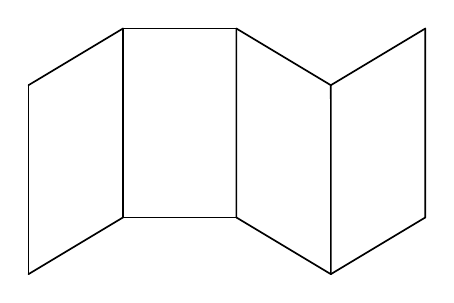
\begin{tikzpicture}[>=latex,scale=1.2,inner sep=1pt]
  \tkzDefPoints{0/0/A,1/0.6/B,2.2/0.6/C,3.2/0/D,4.2/0.6/E,0/2/A'}
  \tkzDefPointsBy[translation=from A to A'](B,C,D,E){B',C',D',E'}
  \tkzDrawSegments[semithick](A,A' B,B' C,C' D,D' E,E' A,B B,C C,D D,E A',B' B',C' C',D' D',E')
\end{tikzpicture}
\end{document}